\chapter{PROBLEM STATEMENT AND SOLUTION PROPOSAL}
\label{ch:chap2}
In this chapter, we will state the problem and show a solution...
\section{Problem}
\subsection{Limited and out date source of bus information}
	The public transportation network has grown over the years in many cities of Vietnam,
	There is only some sources of bus information, but only for some big cities such as Hanoi, Ho Chi Minh city. However, these information is usually misrepresented and out dated data.
	For example, this is the official website for Ho Chi Minh city bus from Ho Chi Minh City department of transport, they only have a few information:
	\begin{figure}[H]
		\centering
		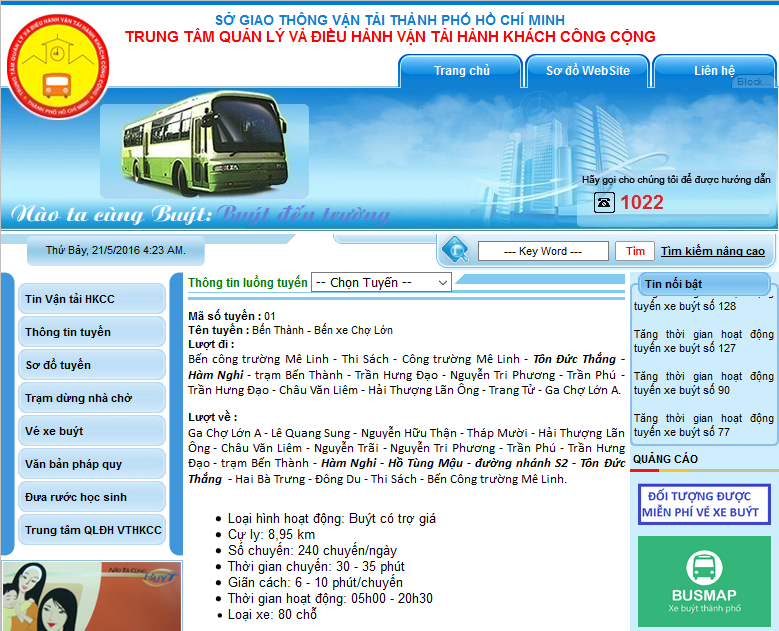
\includegraphics[scale=0.5]{Chapters/Fig/buyttphcm-official}
		\caption{Official website of Ho Chi Minh City department of transport}
		\label{fig:official_website_of_HCMC_department_of_transport}
	\end{figure}
	In many other cities informal public transport systems are operated by independent companies. Often there are no official maps for these systems and little information about them is available.
\subsection{Limited bus application}
	
\section{Requirements}
With above problems
\subsection{Always up-to-date bus information}
\subsection{Mobile application with fully function}


\section{Solution proposal}
From the requirements of the thesis and analysis of related concepts, technologies and researches, 
\subsection{A mobile application client with basic functions and collect data functions}
\subsection{A web service to interact with mobile client}
\subsection{A management application for manage buses route information, process collected data}


\section{Literature review}
\subsection{Concept}
\subsubsection{Crowdsourcing}
	Concept about crowdsourcing...
\subsection{Technology}
\subsubsection{Crowdsourcing}
	\textit{Crowdsourcing}, a modern business term coined in 2006, is defined by Merriam-Webster as the process of obtaining needed services, ideas, or content by soliciting contributions from a large group of people, especially an online community, rather than from employees or suppliers. The word is a combination of the words \'crowd\' and \'outsourcing\'. The idea is to take work and outsource it to a crowd of workers.

	Famous Example: Wikipedia. Instead of Wikipedia creating an encyclopedia on their own, hiring writers and editors, they gave a crowd the ability to create the information on their own. The result? The most comprehensive encyclopedia this world has ever seen.

	Crowdsourcing \& Quality: The principle of crowdsourcing is that more heads are better than one. By canvassing a large crowd of people for ideas, skills, or participation, the quality of content and idea generation will be superior.

	In our thesis, crowdsourcing means we collect bus data from bus passenger, who directly travel by bus. That will be the most correct and up-to-date bus information source.
\subsubsection{Java RESTful web service}
	RESTful web services are built to work best on the Web. Representational State Transfer (REST) is an architectural style that specifies constraints, such as the uniform interface, that if applied to a web service induce desirable properties, such as performance, scalability, and modifiability, that enable services to work best on the Web. In the REST architectural style, data and functionality are considered resources and are accessed using Uniform Resource Identifiers (URIs), typically links on the Web. The resources are acted upon by using a set of simple, well-defined operations. The REST architectural style constrains an architecture to a client/server architecture and is designed to use a stateless communication protocol, typically HTTP. In the REST architecture style, clients and servers exchange representations of resources by using a standardized interface and protocol.

		\begin{figure}[H]
			\centering
			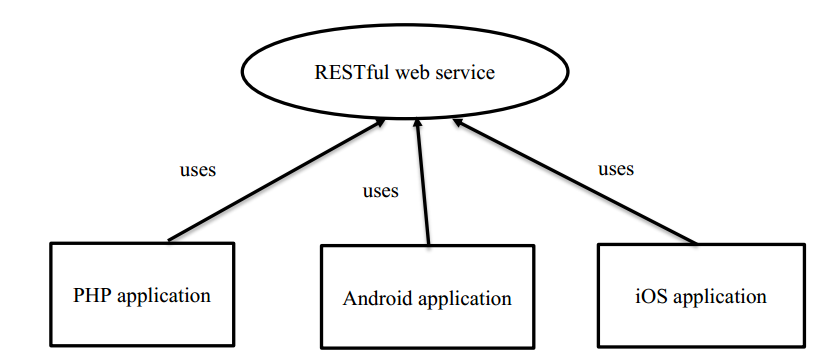
\includegraphics[scale=0.7]{Chapters/Fig/restfull-overview.png}
			\caption{RESTfull overview}
			\label{fig:RESTfull_overview}
		\end{figure}
	In our thesis, we have to build a server that can accept post collected data from client and other interactions with client such as get bus information, update data and more... We chose Java RESTfull web service, because Java RESTful makes it easier to write web applications that apply some or all of the constraints of the REST style to induce desirable properties in the application, such as loose coupling (evolving the server is easier without breaking existing clients), scalability (start small and grow), and architectural simplicity (use off-the-shelf components, such as proxies or HTTP routers). You would choose to use JAX-RS for your web application because it is easier for many types of clients to consume RESTful web services while enabling the server side to evolve and scale. Clients can choose to consume some or all aspects of the service and mash it up with other web-based services. 

	\begin{figure}[H]
		\centering
		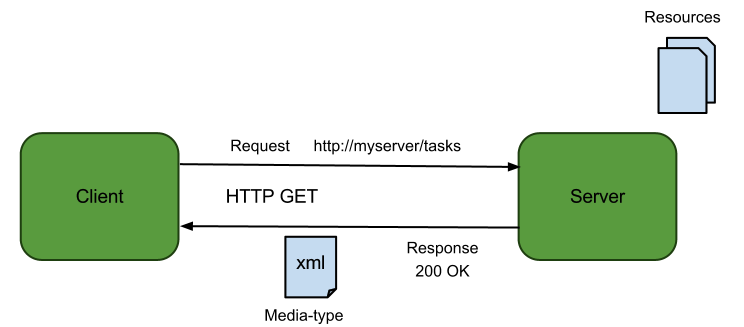
\includegraphics[scale=0.5]{Chapters/Fig/RESTful-Service-Client-Example-Crunchify-Tutorial.png}
		\caption{Java RESTful diagram}
		\label{fig:restful_diagram}
	\end{figure}

\subsubsection{.NET Technology}
	.NET Framework is a software framework developed by Microsoft that runs primarily on Microsoft Windows. It includes a large class library known as Framework Class Library (FCL) and provides language interoperability (each language can use code written in other languages) across several programming languages. Programs written for .NET Framework execute in a software environment (as contrasted to hardware environment) known as Common Language Runtime (CLR), an application virtual machine that provides services such as security, memory management, and exception handling. (As such, computer code written using .NET Framework is called \"managed code\".) FCL and CLR together constitute .NET Framework.

\subsubsection{Windows Phone development kit}

	\paragraph{Windows Phone} Windows Phone is the operating system that runs on Windows Phone devices. The operating system manages the device hardware and provides the technologies required to implement native apps. The operating system also ships with various system apps, such as Phone, Mail, and Safari, which provide standard system services to the user.

		\begin{figure}[H]
			\centering
			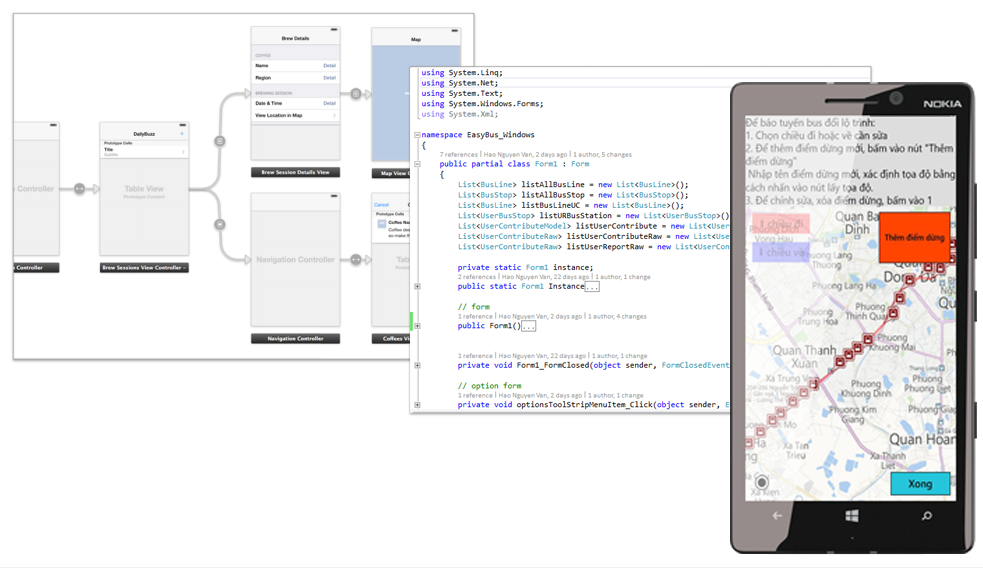
\includegraphics[scale=0.4]{Chapters/Fig/Windows-Phone-development-kit.png}
			\caption{Windows Phone Development Kit}
			\label{fig:wp_dev_kit}
		\end{figure}

	\paragraph{Databinding} Databinding is the process that establishes a connection between the application UI and business logic. If the binding has the correct settings and the data provides the proper notifications, then, when the data changes its value, the elements that are bound to the data reflect changes automatically. Data binding can also mean that if an outer representation of the data in an element changes, then the underlying data can be automatically updated to reflect the change. 
		\begin{figure}[H]
			\centering
			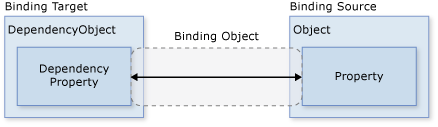
\includegraphics[scale=0.7]{Chapters/Fig/data-binding.png}
			\caption{Data Binding Concept}
			\label{fig:data_binding_concept}
		\end{figure}

	\paragraph{MVVM Pattern} Model–view–viewmodel (MVVM), was developed by Microsoft, facilitates a separation of development of the graphical user interface - be it via a markup language or GUI code - from development of the business logic or back-end logic (the data model). The view model of MVVM is a value converter; meaning the view model is responsible for exposing (converting) the data objects from the model in such a way objects are easily managed and presented. In this respect, the view model is more model than view, and handles most if not all of the view's display logic. The view model may implement a mediator pattern, organizing access to the back-end logic around the set of use cases supported by the view.
		\begin{figure}[H]
			\centering
			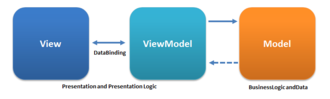
\includegraphics[scale=1.2]{Chapters/Fig/MVVMPattern.png}
			\caption{MVVM Pattern}
			\label{fig:mvvm_pattern}
		\end{figure}
	Components of MVVM pattern
	\begin{itemize}
		\item \textbf{Model}: Model refers either to a domain model, which represents real state content (an object-oriented approach), or to the data access layer, which represents content (a data-centric approach)
		\item \textbf{View}: As in the MVC and MVP patterns, the view is the user interface (UI)
		\item \textbf{View model}: The view model is an abstraction of the view exposing public properties and commands. Instead of the controller of the MVC pattern, or the presenter of the MVP pattern, MVVM has a binder. In the view model, the binder mediates communication between the view and the data binder.[clarification needed] The view model has been described as a state of the data in the model.
		\item \textbf{Binder}: Declarative data- and command-binding are implicit in the MVVM pattern. In the Microsoft solution stack, the binder is a markup language called XAML.[8] The binder frees the developer from being obliged to write boiler-plate logic to synchronize the view model and view. When implemented outside of the Microsoft stack the presence of a declarative databinding technology is a key enabler of the pattern.
	\end{itemize}

\subsection{Related works}
	
\section{Conclusion}
In part 1 of the thesis, I have introduced to ...

% \subsubsection{\acrfull{ced}}
% The main purpose of edge detection is to obtain structure properties of the image with least data extracted for further image processing \cite{canny}. Among some algorithms existing, I choose the one developed by John F. Canny (JFC) \nocite{jfc_canny}. Known as Canny Edge detector or optimal detector, Canny algorithm has three main advantages \cite{code_canny}:
% 	\begin{itemize}
% 		\item \textbf{Low error rate}: Meaning a good detection of only existent edges.
% 		\item \textbf{Good localization}: The distance between edge pixels detected and real edge pixels have to be minimized.
% 		\item \textbf{Minimal response}: Only one detector response per edge.
% 	\end{itemize}

% \subsubsection{\acrshort{ced} algorithm steps}
% \label{sec:ced_step}
% \begin{enumerate}
% 	\item \textbf{Noise filter}: Using Gaussian filter \nocite{gauss_filter}, a sample kernel of \textit{size = 5} might be shown as Equation \ref{eq:gauss}:
% 	\begin{equation}
% 		\label{eq:gauss}
% 		B = \frac{1}{159} .
% 		\left[ \begin{array}{ccccc}
% 		2 & 4 & 5 & 4 & 2 \\
% 		5 & 12 & 15 & 12 & 5 \\
% 		4 & 9 & 12 & 9 & 4 \\
% 		2 & 4 & 5 & 4 & 2
% 		\end{array} \right]
% 	\end{equation}

% 	\item \textbf{Find the intensity gradient of the image}: Gradients at each pixel in the smoothed image are determined by applying Sobel-operator \cite{sobel_alg}:

% 	Apply a pair of convolution masks (in \textit{x} and \textit{y} directions:
% 	\begin{equation}
% 		\label{eq:gx_gy}
% 		G_x =
% 		\left[ \begin{array}{ccc}
% 		-1 & 0 & 1 \\
% 		-2 & 0 & 2 \\
% 		-1 & 0 & 1
% 		\end{array} \right]
% 		\qquad
% 		G_y =
% 		\left[ \begin{array}{ccc}
% 		1 & 2 & 1 \\
% 		0 & 0 & 0 \\
% 		-1 & -2 & -1
% 		\end{array} \right]
% 	\end{equation}

% 	Find the gradient strength and direction with:
% 	\begin{equation}
% 		\label{eq:gradient}
% 		G = \sqrt{G^2_x + G^2_y}
% 	\end{equation}
% 	\begin{equation}
% 		\label{eq:direction}
% 		\theta = arctan\left(\frac{G_y}{G_x}\right)
% 	\end{equation}
% 	The direction is rounded to one of four possible angles (namely 0, 45, 90 or 135)

% 	\item \textbf{Apply Non-maximum suppression}: Removing pixels that are not considered to be part of an edge.
% 	\item \textbf{Double thresholding}: Potential edges are determined by thresholding.
% 	\item \textbf{Edge tracking by hysteresis}: Final edges are determined by suppressing all edges that are not connected to a very certain (strong) edge.
% \end{enumerate}

% \subsection{Shape detection}
% \label{sec:shape_detect}
% The output of \acrshort{ced} process in Section \ref{sec:ced_step} is calculated to decide whether image contains simple geometric shapes (such as triangles, rectangles, squares, pentagons) or not.

% For each edge, contour is retrieved for detecting process. Only contours with area greater than certain amount are considered. Practically, contours larger than 250 pixel are accepted.

% Next, shape of the contour is decided by its attributes. For example, if the contour has 3 vertices, it is a triangle. Correspondingly, a contour has 4 vertices which all the angles in the contour are from 80 to 100 degree is a rectangle.

% \subsection{Text detection and extraction}
% \label{sec:text_detect}
% Mobile phone screen is composed of much of text. Almost object in the screen has text with it. Text segmentation and recognition help the system to understanding the sense of the screen content.

% Our system aims at the automatic detection of text. This is done by the algorithm. Figure \ref{fig:flow_diagram_morph} shows the flow diagram of text detection algorithm. The algorithm steps are summarized as follows.

% \begin{enumerate}
% 	\item An Sobel edge detection scheme is applied to the gray scale image. The image I is blurred (to reduce false edges and over-segmentation) using open-close and close-open filters.
% 	The final blurred image Ib is the average of the outputs of these filters. The 3 x 3 8-connected structuring element of type ``square'' is used here.

% 	Next, the morphological gradient operator \nocite{morph} is applied to the blurred image Ib resulting in an image G as follows:
% 	\begin{center}
% 	G = Dilation (Ib) – Erosion (Ib)
% 	\end{center}

% 	The Morphological gradient is an edge-strength extraction operator that gives symmetric edges between foreground and background regions.

% 	The resulting image is then thresholded to obtain a binary edge image. Otsu and binary thresholding technique is used
% 	for that. \nocite{otsu}

% 	\item Closed edges in the binary edge image are grouped by dilation using eight- connected structuring elements.

% 	Then small connected components in the dilated image are filtered using erosion. The output is a binary image
% 	that contains text candidate regions.

% 	\item Connected component labeling is performed to label each object separately.

% 	\item After applying connected component labeling, the first set of criteria is applied which eliminate all objects whose area is greater than 10000 and filled area is greater than 8000.
% 	One more criteria namely major axis length is used which is used to retain the text region alone.
% 	All objects, whose major axis lengths are in between 20 to 3000, are considered to be text.
% 	To eliminate small objects, connected component labeling is applied to the resultant image and the second set of criteria is applied which eliminates all the objects whose area is less than 300 and filled area is less than 500.
% \end{enumerate}

% After applying all these 4 steps, we get a filtered image that contains only text regions \cite{text_detect}.

% 	\begin{figure}[H]
% 		\centering
% 		\includegraphics{Chapters/Fig/flow_diagram_morph.png}
% 		\caption{Flow diagram of Text Detection algorithm}
% 		\label{fig:flow_diagram_morph}
% 	\end{figure}

% \subsection{\acrlong{ocr}}
% \label{sec:ocr}
% By definition, \acrfull{ocr} is the process or technology of reading data in printed form by a device (optical character reader) that scans and identifies characters \cite{ocr_def}.

% Tesseract is an open-source \acrshort{ocr} engine having comparative recognition accuracy. Originally developed by HP between 1984 and 1994, Tesseract became open-source in 2005 and is developed by Google since 2006 \cite{ocr_overview}. According to 1995 UNLV results, Tesseract can achieve accuracy up to 98\% on English newspaper \cite{Rice_thefourth}.

% Figure \ref{fig:tesseract_arch} briefly describes the architecture of Tesseract \acrshort{ocr} engine \cite{tesseract_oscon}:

% 	\begin{figure}[H]
% 		\centering
% 		\includegraphics[scale=0.5]{Chapters/Fig/tesseract_arch.png}
% 		\caption{Tesseract \acrshort{ocr} Architecture}
% 		\label{fig:tesseract_arch}
% 	\end{figure}

% The output results of this phrase are used for naming objects which are identified in later script processing steps that we will discover in next chapter.

% \section{Recognition result}
% This section presents the result of unit testing for each image processing function of Image Processor component.

% \subsection{Button detection}
% Buttons are detected by their shape using technique presented in Section \ref{sec:shape_detect}.

% 	\begin{figure}[H]
% 	    \centering
% 	    \subfigure{
% 	        \centering
% 	        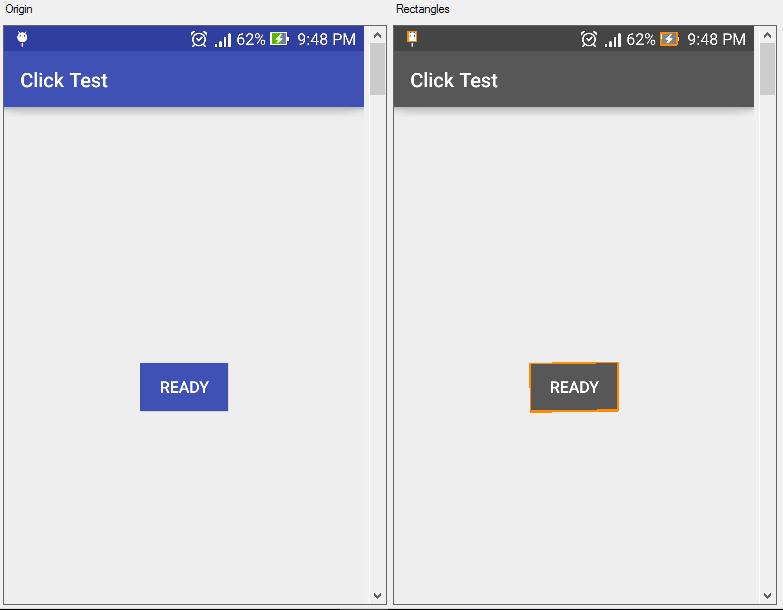
\includegraphics[scale=0.5]{Chapters/Fig/rect_detect.png}
% 	    }
	    
% 	    \subfigure{
% 	        \centering
% 	        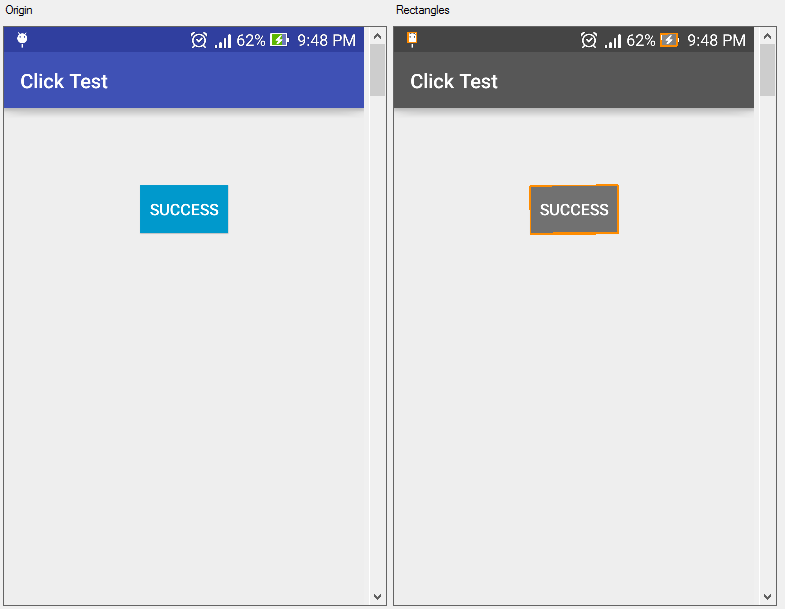
\includegraphics[scale=0.5]{Chapters/Fig/rect_detect_2.png}
% 	    }

% 	    \caption{Button detection result}
% 		\label{fig:btn_detect}
% 	\end{figure}

% \subsection{Text detection}
% Text is detected and segmented by algorithm in Section \ref{sec:text_detect}

% 	\begin{figure}[H]
% 	    \centering
% 	    \subfigure[Text detection in alarm home screen]{
% 	        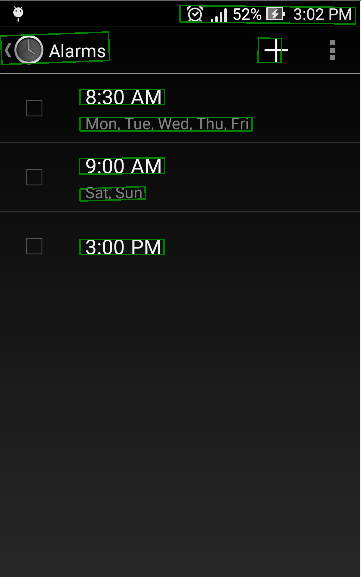
\includegraphics[scale=0.5]{Chapters/Fig/text_detect_home.png}
% 	    }
% 	    \qquad
% 	    \subfigure[Text detection in alarm item screen]{
% 	        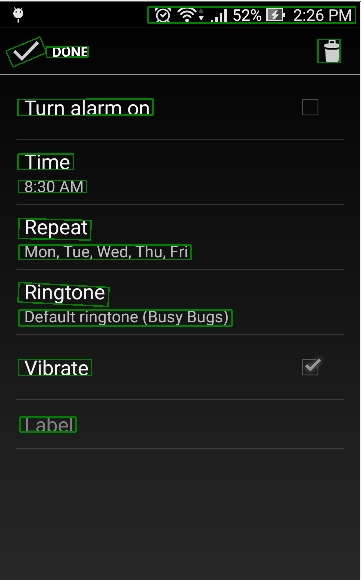
\includegraphics[scale=0.5]{Chapters/Fig/text_detect_item.png}
% 	    }
% 	    \qquad
% 	    \subfigure[Text detection in alarm time select screen]{
% 	        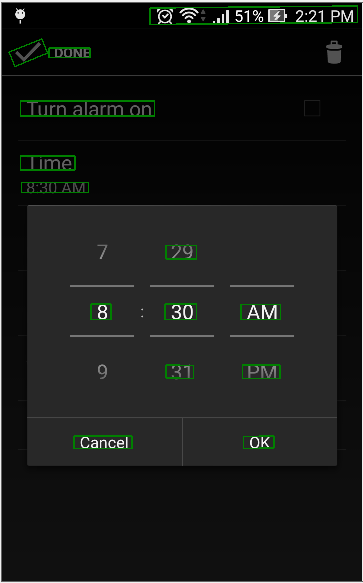
\includegraphics[scale=0.5]{Chapters/Fig/text_detect_clock.png}
% 	    }
% 	    \qquad
% 	    \caption{Text detection result}
% 		\label{fig:text_detect}
% 	\end{figure}

% \subsection{Keyboard detection}
% Keyboard consists of rectangle buttons. This feature shares the same detection method with Button detection.

% 	\begin{figure}[H]
% 		\centering
% 		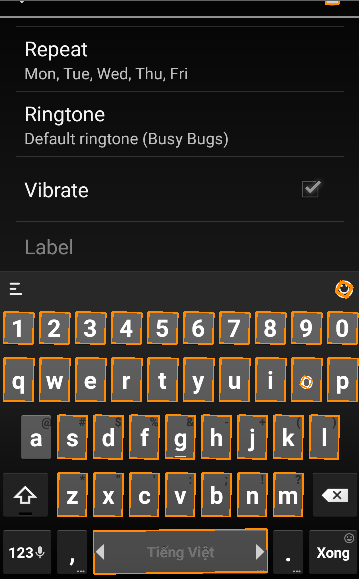
\includegraphics[scale=0.5]{Chapters/Fig/kb_detect.png}
% 		\caption{Keyboard detection result}
% 		\label{fig:kb_detect}
% 	\end{figure}

% \subsection{\acrlong{ocr}}
% Text segments detected in previous section is used for recognizing process. After this stage, object will have a name given from recognized text and a relative location on the screen.

% 	\begin{figure}[H]
% 	    \centering
% 	    \subfigure[Text recognition in alarm home screen]{
% 	        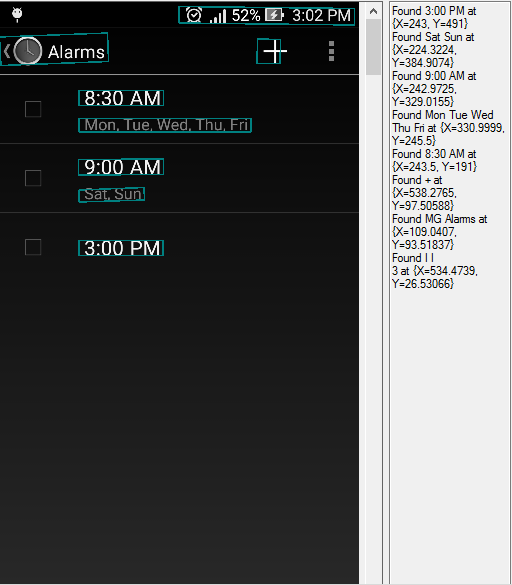
\includegraphics[scale=0.5]{Chapters/Fig/found_home.png}
% 	    }
% 	    \qquad
% 	    \subfigure[Text recognition in alarm item screen]{
% 	        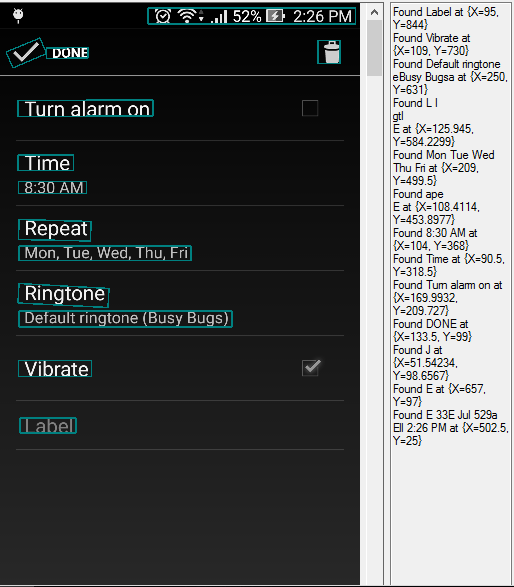
\includegraphics[scale=0.5]{Chapters/Fig/found_item.png}
% 	    }
% 	    \qquad
% 	    \subfigure[Text recognition in alarm time select screen]{
% 	        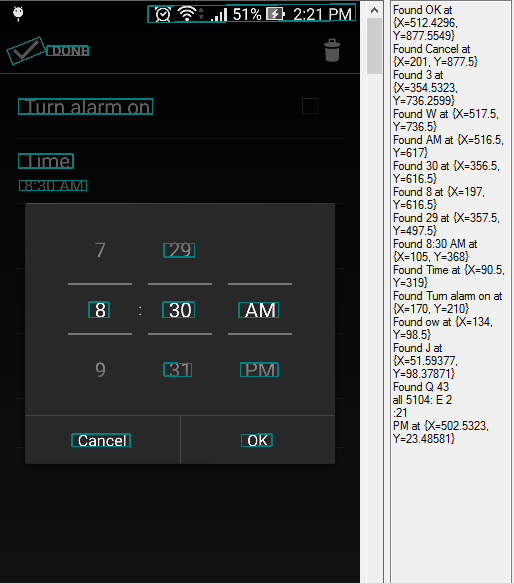
\includegraphics[scale=0.5]{Chapters/Fig/found_clock.png}
% 	    }
% 	    \qquad
% 	    \caption{Text recognition result}
% 		\label{fig:text_recognize}
% 	\end{figure}
